
%(BEGIN_QUESTION)
% Copyright 2011, Tony R. Kuphaldt, released under the Creative Commons Attribution License (v 1.0)
% This means you may do almost anything with this work of mine, so long as you give me proper credit

Examine this cross-limited air/fuel control system, then determine how it will respond to the following faults (assuming a constant 50\% firing command signal):

$$\includegraphics[width=15.5cm]{i01731x01.eps}$$

\begin{itemize}
\item{} Air flow transmitter fails high
\vskip 10pt
\item{} Fuel flow transmitter fails high 
\vskip 10pt
\item{} Air valve fails shut
\vskip 10pt
\item{} Fuel valve fails shut
\end{itemize}

\vskip 20pt \vbox{\hrule \hbox{\strut \vrule{} {\bf Suggestions for Socratic discussion} \vrule} \hrule}

\begin{itemize}
\item{} Perhaps the most important question to ask yourself when analyzing the effects of these faults is {\it how to properly track all the signal values when performing each ``thought experiment''}.  Identify ways you use to keep track of all the signal values as you analyze various faults in this system.
\end{itemize}

\underbar{file i01731}
%(END_QUESTION)





%(BEGIN_ANSWER)


%(END_ANSWER)





%(BEGIN_NOTES)

\begin{itemize}
\item{} Air flow transmitter fails high: {\it air flow shuts off; fuel flow remains at firing command setpoint; fire burns rich (possibly going out)}
\vskip 10pt
\item{} Fuel flow transmitter fails high: {\it fuel flow shuts off; air flow goes to maximum; fire goes out} 
\vskip 10pt
\item{} Air valve fails shut: {\it air and fuel flow both shut off; fire goes out}
\vskip 10pt
\item{} Fuel valve fails shut: {\it fuel flow shuts off; air flow remains at firing command setpoint; fire goes out}
\end{itemize}

%INDEX% Process: combustion furnace
%INDEX% Relay, computational: high select (used in cross-limited air/fuel ratio control system)
%INDEX% Relay, computational: low select (used in cross-limited air/fuel ratio control system)

%(END_NOTES)


